% !TEX root=../report.tex

\section{Performing tasks one after the other}

In the previous section we have set up our interaction model of events and actions,
we defined our interactive component, the editor,
and introduced the infinitely failing task.
Now that we have the core part of an interactive workflow,
we can continue with ways to compose multiple tasks.
Combining tasks can be done in two ways:
\begin{enumerate*}
  \item sequential or
  \item parallel.
\end{enumerate*}
For parallel composition we distinguish two kinds:
\begin{enumerate*}[(a)]
  \item pairing two tasks (\emph{and}-parallel); and
  \item choosing between two tasks (\emph{or}-parallel).
\end{enumerate*}
In this section we start with sequential composition.
The next two sections are about pairing and choosing.

One might think that the best way to sequence tasks is by just following one task with another:
do this, then do that, then that, etc.
However, we like the continuation to depend on the value produced by the preceding task.
\todo{Elaborate more about the reasons for this.}
This is done by a \emph{step}.
We define a step from one task to another as
\begin{quote}
  a calculation which returns the next task to proceed with.
\end{quote}

To accomplish this,
we take continuations to be \emph{functions}.
These are just normal functions from our host language which,
when evaluated, result in something of type $\Task$.
Therefore,
we extend our pretasks $p$ with a sequence construct $\Then$.
\begin{grammar}
  Pretasks
    & p & ::=& \ldots        & \\
    &   &\mid& e_1 \Then e_2 & – step \\
\end{grammar}

The accompanied typing rule looks like
\begin{equation*}
  \userule{T-Then}
\end{equation*}
Note that typing ensures us that the left hand side $e_1$ will be a task delivering a value of type $\tau_1$.
The right hand side $e_2$ then, will use this value of type $\tau_1$,
and calculate a \emph{new} task holding a value of (possibly another) type $\tau_2$.

Evaluation of a sequence is done by only evaluating the left hand side, $e_1$,
as this expression is be something of type $\Task \tau_1$.
As the right hand side, $e_2$, is a function,
it does not matter if we evaluate $e_2$ right away or store it lazily.
\begin{equation*}
  \userule{E-Then}
\end{equation*}
Consequentially, we extend our tasks $t$ with an evaluated sequence construct.
\begin{grammar}
  Tasks
    & t & ::=& \ldots        & \\
    &   &\mid& t_1 \Then e_2 & – sequence \\
\end{grammar}


\subsection{Layered semantics}
\label{sec:normalise}
\label{sec:drive}

Stepping from one task to another using the sequence construct $\Then$ is done by the system itself,
not by the user.
We will call this an \emph{internal step} or \emph{system step}.\footnote{
  This implies there will also be an \emph{external step} or \emph{user step} performed on users' request.
  This is indeed the case and we will discuss it in \autoref{sec:external-step}.
}
As there is no explicit user input needed to perform an internal step,
we cannot use our event handling semantics $\handle{h}$,
described in \autoref{sec:handling},
to specify stepping from one task to the next (calculated) one.
Also,
using our evaluation semantics to do so,
would pollute the semantics our our host language with rules specific for the task layer.

Therefore we introduce another semantic relation which we will call \emph{normalisation}.
When considering our semantic relations as a hierarchy,
normalisation conceptually lies \emph{between} evaluation and handling.
Normalisation will make use of evaluation of our underlying host language and,
as we will see later on,
handling will make use of normalisation
and the functions $\Value(t)$ and $\Succeeding(t)$ from sections \autoref{sec:value} and \autoref{sec:succeeding}.

Graphically,
we now have the following semantic functions shown in \autoref{fig:semantic-functions}.
Note that the double down arrow $\normalise$ \emph{uses} the single down arrow $\evaluate$,
a convention we will use again later in this text.

\begin{figure}
  \centering
  \includegraphics[width=0.6\textwidth,page=4]{figures/drawings-crop.pdf}
  \caption{Semantic functions defined in this report and their relation.}
  \label{fig:semantic-functions}
\end{figure}

As evaluation,
normalisation is a \emph{big step} semantics.
We write $\boxed{\userule{RelationN}}$ to describe that
task $t$ normalises to task $t'$.
Note that, as handling,
normalisation \emph{only acts upon tasks}.
It is a semantic relation that lives \emph{on the task level}.
We can think of normalisation as a \enquote{medium step} semantics,
normalising tasks $t$ as much as possible,
till the moment it needs an event to continue.
For editors and the failing task normalisation is simple.
\begin{equation*}
  \userule{N-Edit} \qquad \userule{N-Fill} \qquad \userule{N-Fail}
\end{equation*}
In the next subsection we will introduce rules to normalise a task sequence.

To ensure tasks are ready to process the next event,
we need to normalise after each use of the handling semantics.
Instead of adding normalisation to every handling rule,
we introduce a fourth semantic relation to deal with this.
The drive relation $\boxed{\RelationD}$ simply passes the event $h$ to the handle semantics
and normalises the task afterwards.
\begin{equation*}
  \userule{D-Main}
\end{equation*}
Note that again,
the double arrow $\drive{h}$ uses the single arrow $\handle{h}$.



\subsection{Two principles of stepping}
\label{sec:normalise-sequence}

Now that we have extended our syntax with a sequencing construct,
and defined its evaluation,
the question to answer is:
\enquote{How do we determine the next task
and when is the time we should proceed proceed with it?}
There are two main principles when stepping from task $t_1$ to task $t_2$:
\begin{enumerate}[S1]
  \item We can only step from a task if it has a value, i.e. $\Value(t_1) = v_1$. \label{itm:step1}
  \item It is not allowed to step to a failing task, i.e. $\Succeeding(t_2)$ holds. \label{itm:step2}
\end{enumerate}

The intuition behind principle \autoref{itm:step1} is simply that we are not able to calculate the next task from a function
when we do not have a value to pass it.
Principle \autoref{itm:step2} protects us from stepping to a failing task,
which comes in hand when specifying guards.
We will show an example of this in \autoref{sec:guards}.

\begin{margintext}{Aside: Failure and stepping}
  In a previous attempt,
  \textcite{theses/radboud/VinterHviid18} used \type{Just} and \type{Nothing}
  to distinguish succeeding and failing tasks.
  This has an unfortunate consequence.
  The type of our sequence combinator changes from
  \begin{equation*}
    \Task \tau_1 \to (\tau_1 \to \Task \tau_2) \to \Task \tau_2
  \end{equation*}
  to
  \begin{equation*}
    \begin{split}
      \Task \tau_1 &\to (\tau_1 \to \Maybe\ (\Task \tau_2))\\
                   &\to \Task \tau_2.
    \end{split}
  \end{equation*}
  This makes it impossible to use the sequencing combinator as a candidate for a monadic bind.
  Lifting an error value directly into the task layer gives us the ability to internally signal failure
  without compromising typing.
\end{margintext}

Above rules imply that we have three cases when normalising a sequence.
First,
it could be the case that the left hand side does not have a value after normalisation.
This means we cannot pass a value to the right hand side
and thus we cannot make the step.
\begin{equation*}
  \userule{N-ThenStay}
\end{equation*}

\begin{margintext}{Aside: Sequencing in iTask}
  Again a side note for the iTasks guru.
  In this section we introduced a way to step from one task to another.
  How does this compare to the step combinators found in the iTasks framework?
  Which combinator does $\Then$ correspond to?

  From the multiple options that we have,
  only \type{(>>=)}, \type{(>>-)} and \type{(>>\texttilde)} have the right type.
  Normalisation rules \refrule{N-ThenStay}, \refrule{N-ThenFail} and \refrule{N-ThenCont} ensure stepping without any user interaction,
  i.e. users are not presented with a continue button.
  Therefore our $\Then$ constructor corresponds mostly to the iTasks \type{(>>-)} combinator.
\end{margintext}

Second,
the normalised left hand side has a value,
but when evaluating the right hand side,
it leads to a failing task.
We do not allow stepping to a failing task
and thus we also cannot make a step.
\begin{equation*}
  \userule{N-ThenFail}
\end{equation*}
Note we use the evaluation semantics of our host language
to evaluate the function application $e_2\ v_1$ to a new task $t_2$.

Third,
the normalised left hand side has a value,
and the evaluated right hand side is a succeeding task.
Now we can make a step!
\begin{equation*}
  \userule{N-ThenCont}
\end{equation*}
Note we normalise $t_2$ first before yielding our result.

The sequence construct itself does not handle any user input.
The left hand side however,
can be an interactive task, such as an editor.
To reach this encapsulated interactive task,
$\Then$ needs to pass events to the left.
\begin{equation*}
  \userule{H-PassThen}
\end{equation*}

Almost there!
We did not extend the functions $\Succeeding(t)$ and $\Value(t)$ for our new sequencing construct $\Then$.
Intuitively,
when we have a task $\Fail \Then e_2$ we are stuck.
As in the case of just the task $\Fail$,
users can send any event,
but nothing will ever happen.
$\Fail$ will never have a value
and therefore $\Then$ will never make a step to $e_2$.\footnote{
  This is a property called \emph{left absorption},
  which tells us something about the interaction between $\Fail$ and $\Then$.
  See also \autoref{sec:monad-laws}.
}
If the left hand side of $\Then$ is any other task,
all will be well.
Thus,
a sequence $t_1 \Then e_2$ is succeeding iff its left hand side $t_1$ is succeeding.
\begin{equation*}
  \begin{array}{lcl}
    \Succeeding(t_1 \Then e_2) &=& \Succeeding(t_1)
  \end{array}
\end{equation*}

The question remains what value we have to associate to a task sequence.
The answer is: none!
Imagine the task $t := \Edit \str{Hello} \Then \lambda s.\allowbreak\Edit (\Length s)$,
where a user entered a string and our task gives the length of the string as the result.
Recall the definition of $\Value(t)$ from \autoref{sec:value}.
The value of the left hand side of $t$ is the string $\str{Hello}$.
After stepping to the right hand side,
the value of $t$ should be $\Value(\Edit (\Length\str{Hello})) = \Value(\Edit 5) = 5$.
This means the type of the value \emph{changed} after taking the step.
\todo{Elaborate more about why this is not desirable.}
Therefore we define that a sequence of tasks \emph{does not} have a value.\footnote{
  We could choose that the value of a sequence equals the value of the left hand side.
  This will have fatal consequences for our stepping semantics however.
}
\begin{equation*}
  \begin{array}{lcl}
    \Value(t_1 \Then e_2) &=& \bot
  \end{array}
\end{equation*}


\subsection{Example: conditional stepping}

% \begin{equation*}
%   \Fill \Int \Then \lambda n. \If{n \ge 10}{\Edit \str{large}}{\Fail}
% \end{equation*}

\begin{margintext}{Aside: Conditional stepping in iTasks}
  In iTasks we would write the example on the left using the step combinator
  and a list with an \type{OnValue} specifying the predicate:
  \begin{verbatim}
    enterInformation "" [] >>* [
      OnValue
        (ifValue $ \n -> n >= 10)
        (const $ return "large"))
    ]
  \end{verbatim}
\end{margintext}

\begin{align*}
    & \Fill \Int \Then \lambda n. \If{n \ge 10}{\Edit \str{large}}{\Fail} \\
  \drive{8} & \hint{change value to eight, rhs evaluates to $\Fail$} \\
    & \Edit 8 \Then \lambda n. \If{n \ge 10}{\Edit \str{large}}{\Fail} \\
  \drive{3} & \hint{change value to three, rhs still failing} \\
    & \Edit 3 \Then \lambda n. \If{n \ge 10}{\Edit \str{large}}{\Fail} \\
  \drive{12} & \hint{change value to twelve, rhs succeeds now!} \\
    & \Edit \str{large}
\end{align*}


\subsection{Intermezzo: monad and its laws}
\label{sec:monad-laws}

To be able to investigate properties about tasks,
we need some notion of equality.
Of course there is syntactic equality,
denoted $t_1 \equiv t_2$,
which is obviously too strong.
We define a new relation $t_1 \approxeq t_2$,
which we read as \enquote{$t_1$ is \emph{normalised equal} to $t_2$} as follows.
\todo{This is wrong! It makes $\Fill \beta$ and $\Fail$ equivallent.}
\begin{equation*}
  \begin{array}{crc}
    t_1 \approxeq t_2 &\text{if and only if}& t_1 \normalise t_1' \\
                      &\text{and}           & t_2 \normalise t_2' \\
                      &\text{and}           & \Value(t_1') = \Value(t_2') \\
  \end{array}
\end{equation*}
We demand that \emph{the values of both tasks after normalisation should be equal}.
% Note that, again, the double waved relation $\approxeq$ uses the single waved relation $\simeq$.
% For now,
% think of $v_1 \simeq v_2$ as syntactic equality on values.
% We will make this more specify this later on.

Sequencing together with editors form a monad.
Here, $\Then$ poses as the well know bind operation,
and $\Edit$ poses as pure.
We have the following laws for \emph{type correct expressions}.
\begin{equation*}
  \begin{array}{rclr}
    \Edit x \Then g
      &\approxeq& g\ x
      & \text{(left identity)} \\
    t \Then\ (\lambda y. \Edit y)
      &\approxeq& t
      & \text{(right identity)} \\
    (t \Then g) \Then h
      &\approxeq& t \Then\ (\lambda y. g\ y \Then h)
      & \text{(associativity)}
  \end{array}
\end{equation*}

Left identity follows quite naturally from the rules in \autoref{sec:normalise-sequence}.
As $\Edit x$ has a value,
\refrule{N-ThenCont} will step to the right hand side and evaluate $g\ x$.

Right identity is a bit harder to see at once.
We have two cases.
\begin{enumerate*}
  \item
    When $\Value(t) = \bot$ we cannot make a step, by \refrule{N-ThenStay},
    and $\Value(t \Then \lambda x. \Edit x)$ is also $\bot$.
  \item
    When $\Value(t) = v$ we can make a step.
    Now, we need to show that $\Edit v \approxeq t$.
    Checking the definition of $\Value(t)$,
    we could only make a step when $t = \Edit v$.\footnote{
      A similar argument will hold for $t_1 \And t_2$ and $t_1 \Or t_2$,
      when we add this to our task layer later in this report.
    }
    Thus we have $\Edit v \approxeq \Edit v$ which clearly holds.
\end{enumerate*}

Associativity holds with a similar argument.
\todo{Elaborate more.}


\subsection{Proceeding on users' request}

\begin{grammar}
  Pretasks
    & p & ::=& \ldots        & \\
    &   &\mid& e_1 \Next e_2 & – user step \\
  Tasks
    & t & ::=& \ldots        & \\
    &   &\mid& t_1 \Next e_2 & – user step \\
\end{grammar}

Rules are similar to those for $\Then$,
only \refrule{H-Next} is new and specific for external stepping.

\begin{equation*}
  \userule{T-Next}
\end{equation*}

\begin{equation*}
  \userule{E-Next}
\end{equation*}

\begin{margintext}{Aside: User steps and iTasks}
  $\Next$ is similar to \type{>>=}.
\end{margintext}

\begin{equation*}
  \userule{N-Next}
\end{equation*}

\begin{equation*}
  \begin{array}{lcl}
    \Value(t_1 \Next e_2) &=& \bot
  \end{array}
\end{equation*}

\begin{equation*}
  \begin{array}{lcl}
    \Succeeding(t_1 \Next e_2) &=& \Succeeding(t_1)
  \end{array}
\end{equation*}

\begin{grammar}
  Actions
    & a & ::=& \ldots & \\
    &   &\mid& \Continue  & – continue with next task \\
\end{grammar}

\begin{equation*}
  \userule{H-PassNext}
\end{equation*}

\begin{equation*}
  \userule{H-Next}
\end{equation*}


\subsection{Example: waiting for users to continue}

\begin{margintext}{Aside: External step in iTasks}
  In iTasks we would write the example on the left using the \type{>>=} combinator:
  \begin{verbatim}
    enterInformation  "" []   >>= \x ->
    updateInformation "" [] 2 >>= \y ->
    return (x + y)
  \end{verbatim}
\end{margintext}

\begin{align*}
    & \Fill \Int \Next \lambda x. \Edit 2 \Next \lambda y. \Edit (x + y) \\
  \drive{4} & \hint{change value to four, we do not step automatically} \\
    & \Edit 4 \Next \lambda x. \Edit 2 \Next \lambda y. \Edit (x + y) \\
  \drive{\Continue} & \hint{hit continue, now step, but just once} \\
    & \Edit 2 \Next \lambda y. \Edit (4 + y) \\
  \drive{7} & \hint{change default value to seven} \\
    & \Edit 7 \Next \lambda y. \Edit (4 + y) \\
  \drive{\Continue} & \hint{hit continue, now step} \\
    & \Edit 11 \\
\end{align*}
